\documentclass[12pt,a4paper,leqno]{report}

\usepackage[T1]{fontenc}
\usepackage[english]{babel}
\usepackage{amsthm}
\usepackage{amsfonts}
\usepackage{amsmath}
\usepackage{amssymb}
\usepackage{tikz}
\usepackage{listings}

\newcommand{\R}{\mathbb{R}}
\newcommand{\C}{\mathbb{C}}
\newcommand{\Q}{\mathbb{Q}}
\newcommand{\N}{\mathbb{N}}
\newcommand{\No}{\mathbb{N}_0}
\newcommand{\Z}{\mathbb{Z}}
\newcommand{\diam}{\operatorname{diam}}

\theoremstyle{plain}
\newtheorem{equa}[equation]{Equation}
\newtheorem{lem}[equation]{Lemma}
\newtheorem{prop}[equation]{Proposition}
\newtheorem{cor}[equation]{Corollary}

\theoremstyle{definition}
\newtheorem{defi}[equation]{definition}
\newtheorem{conj}[equation]{Conjecture}
\newtheorem{example}[equation]{Example}

\theoremstyle{remark}
\newtheorem{note}[equation]{Note}

\pagestyle{plain}
\makeatletter
\renewcommand{\@seccntformat}[1]{}
\makeatother
\setcounter{page}{1}
\addtolength{\hoffset}{-1.15cm}
\addtolength{\textwidth}{2.3cm}
\addtolength{\voffset}{0.45cm}
\addtolength{\textheight}{-0.9cm}

\graphicspath{ {./figures/} }

\title{Data Analytics 2 - Predicting Brand Preference}
\author{Tuomo Kareoja}
\date{}

\begin{document}

\maketitle

\begin{table}[h!]
  \begin{center}
    \caption{Version history}
    \begin{tabular}{l|c|r}
      \textbf{Version Number} & \textbf{Changes} & \textbf{Date} \\
      \hline
      0.1 & Created basic outline without content & 01.08.2019\\
      0.2 & Added visualizations, printouts and text outlines & 02.08.2019\\
    \end{tabular}
  \end{center}
\end{table}

\newpage

\section{Fixed predictions}


\bigskip
{
    \centering
    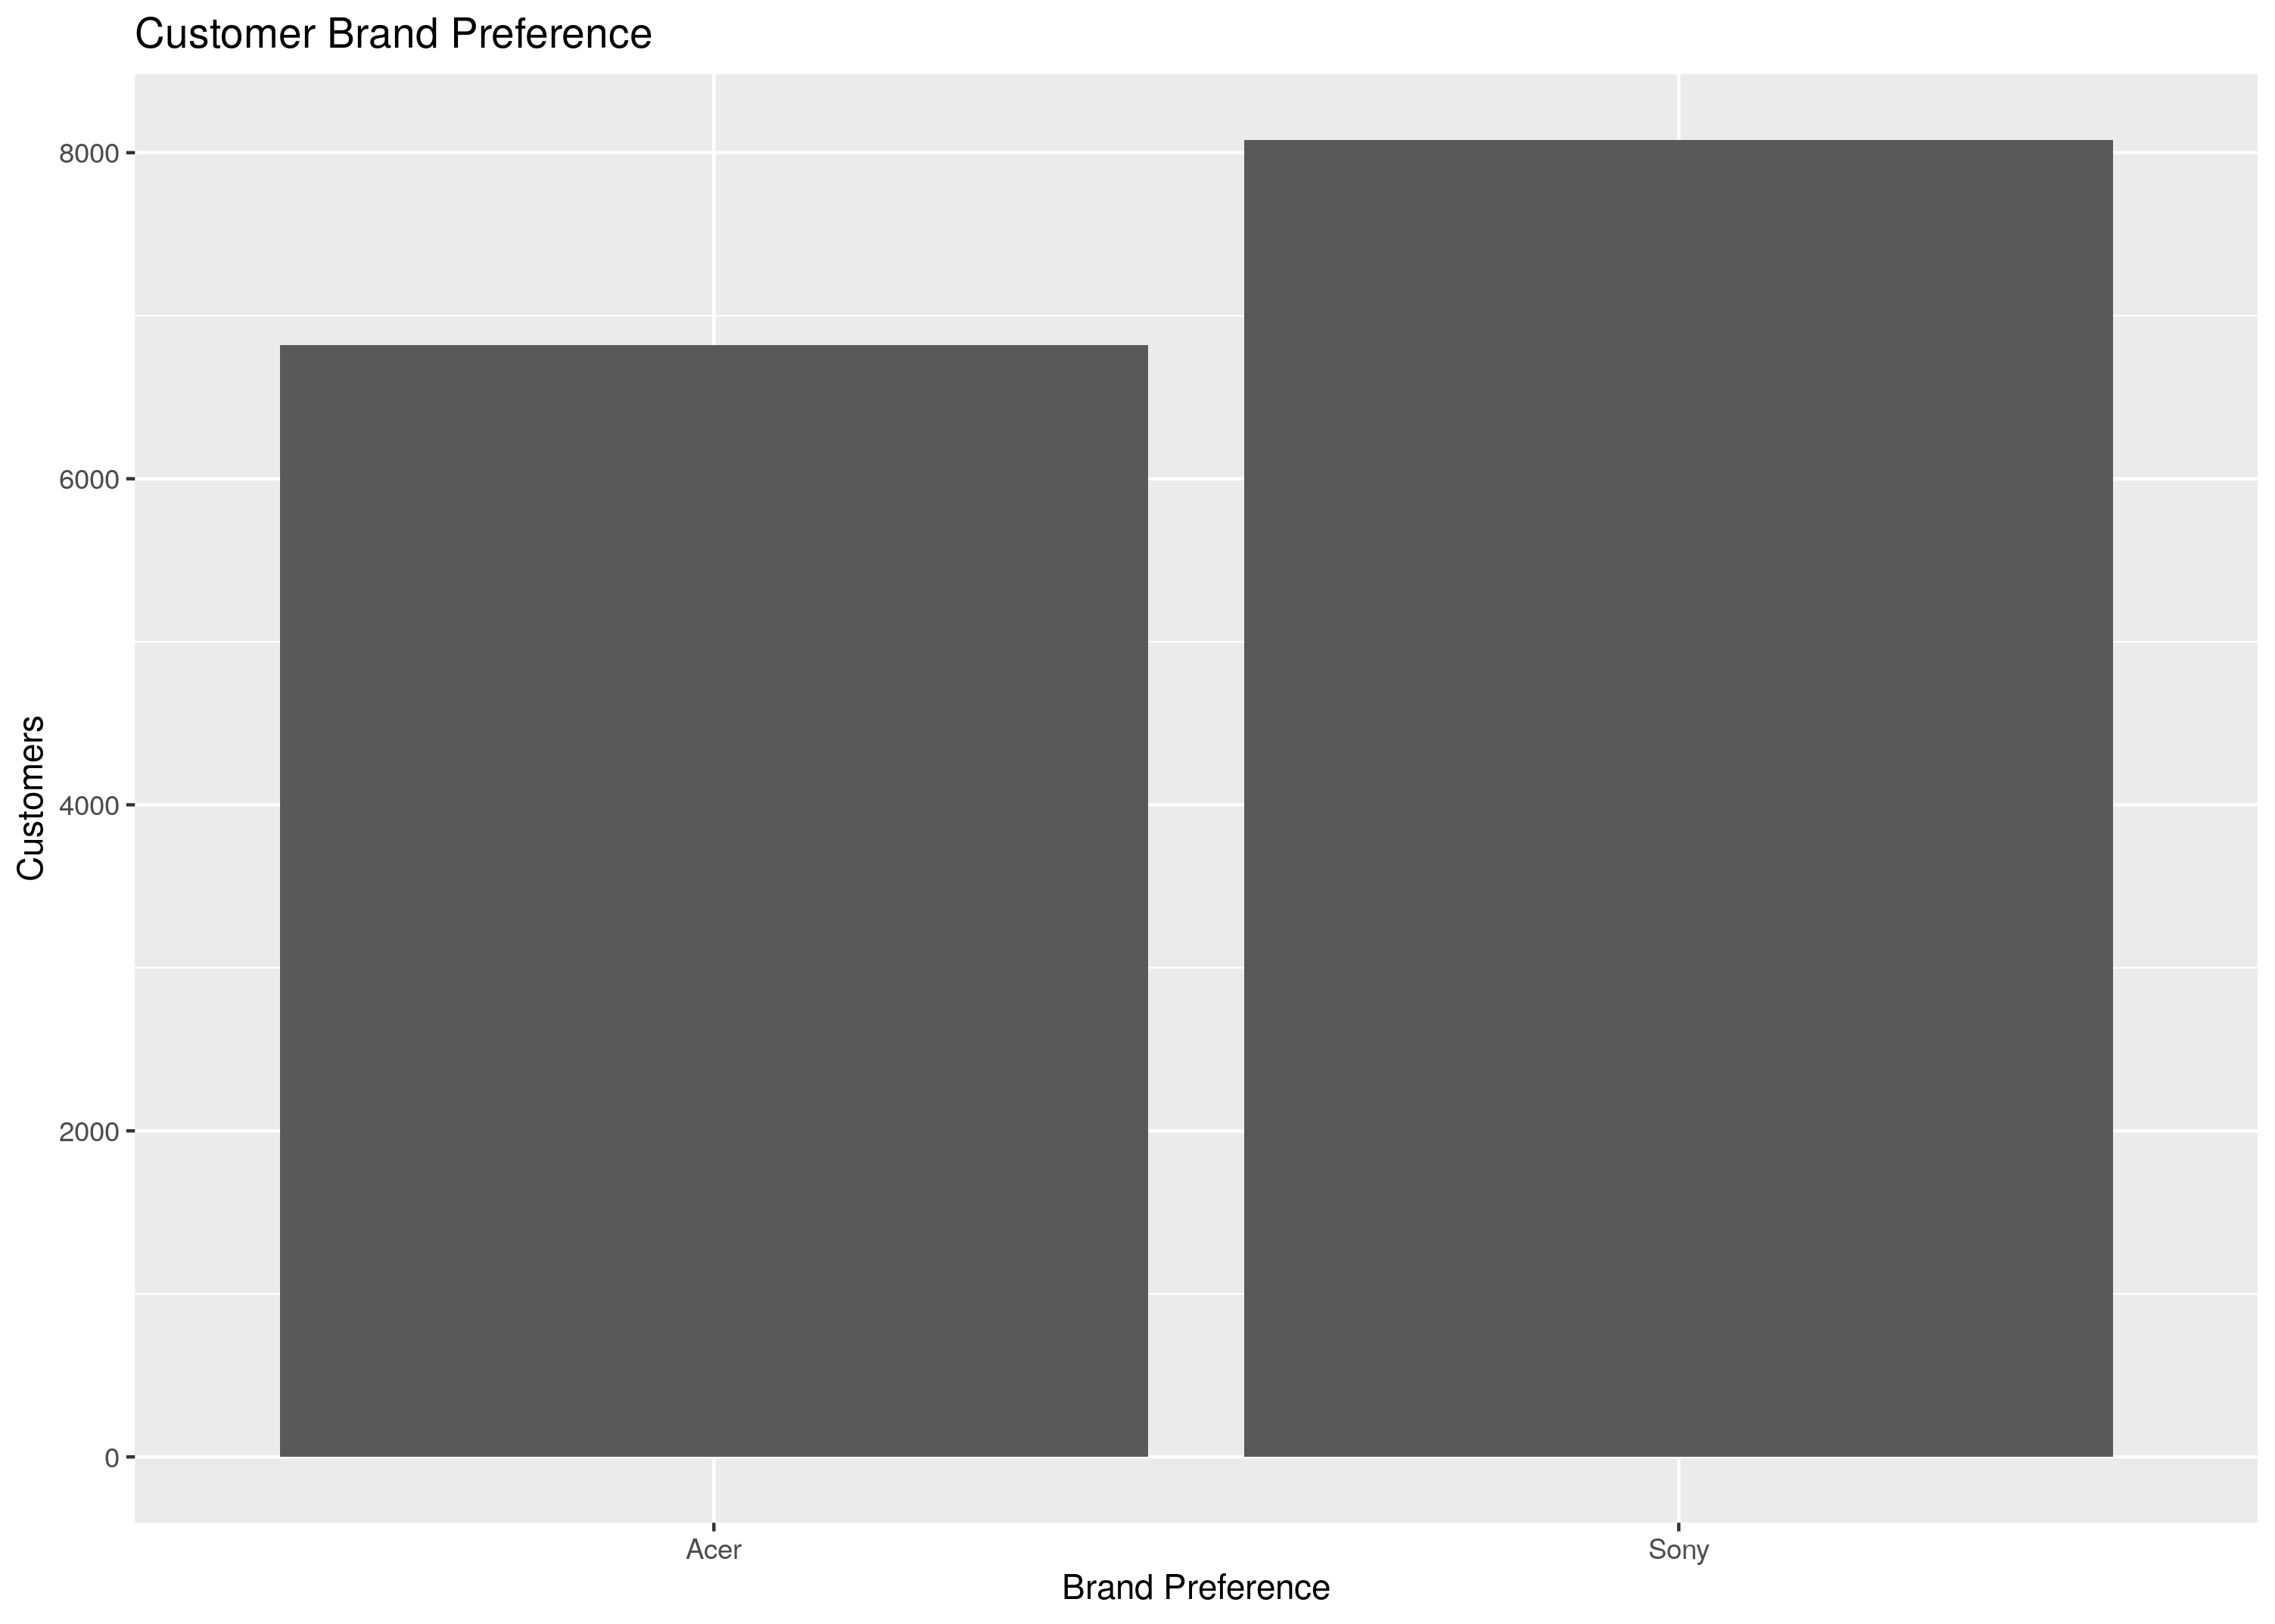
\includegraphics[width=\textwidth,height=\textheight,keepaspectratio]{brand_preference_plain.png}
    \par
}
\bigskip

These are results after we added predictions

\bigskip
{
    \centering
    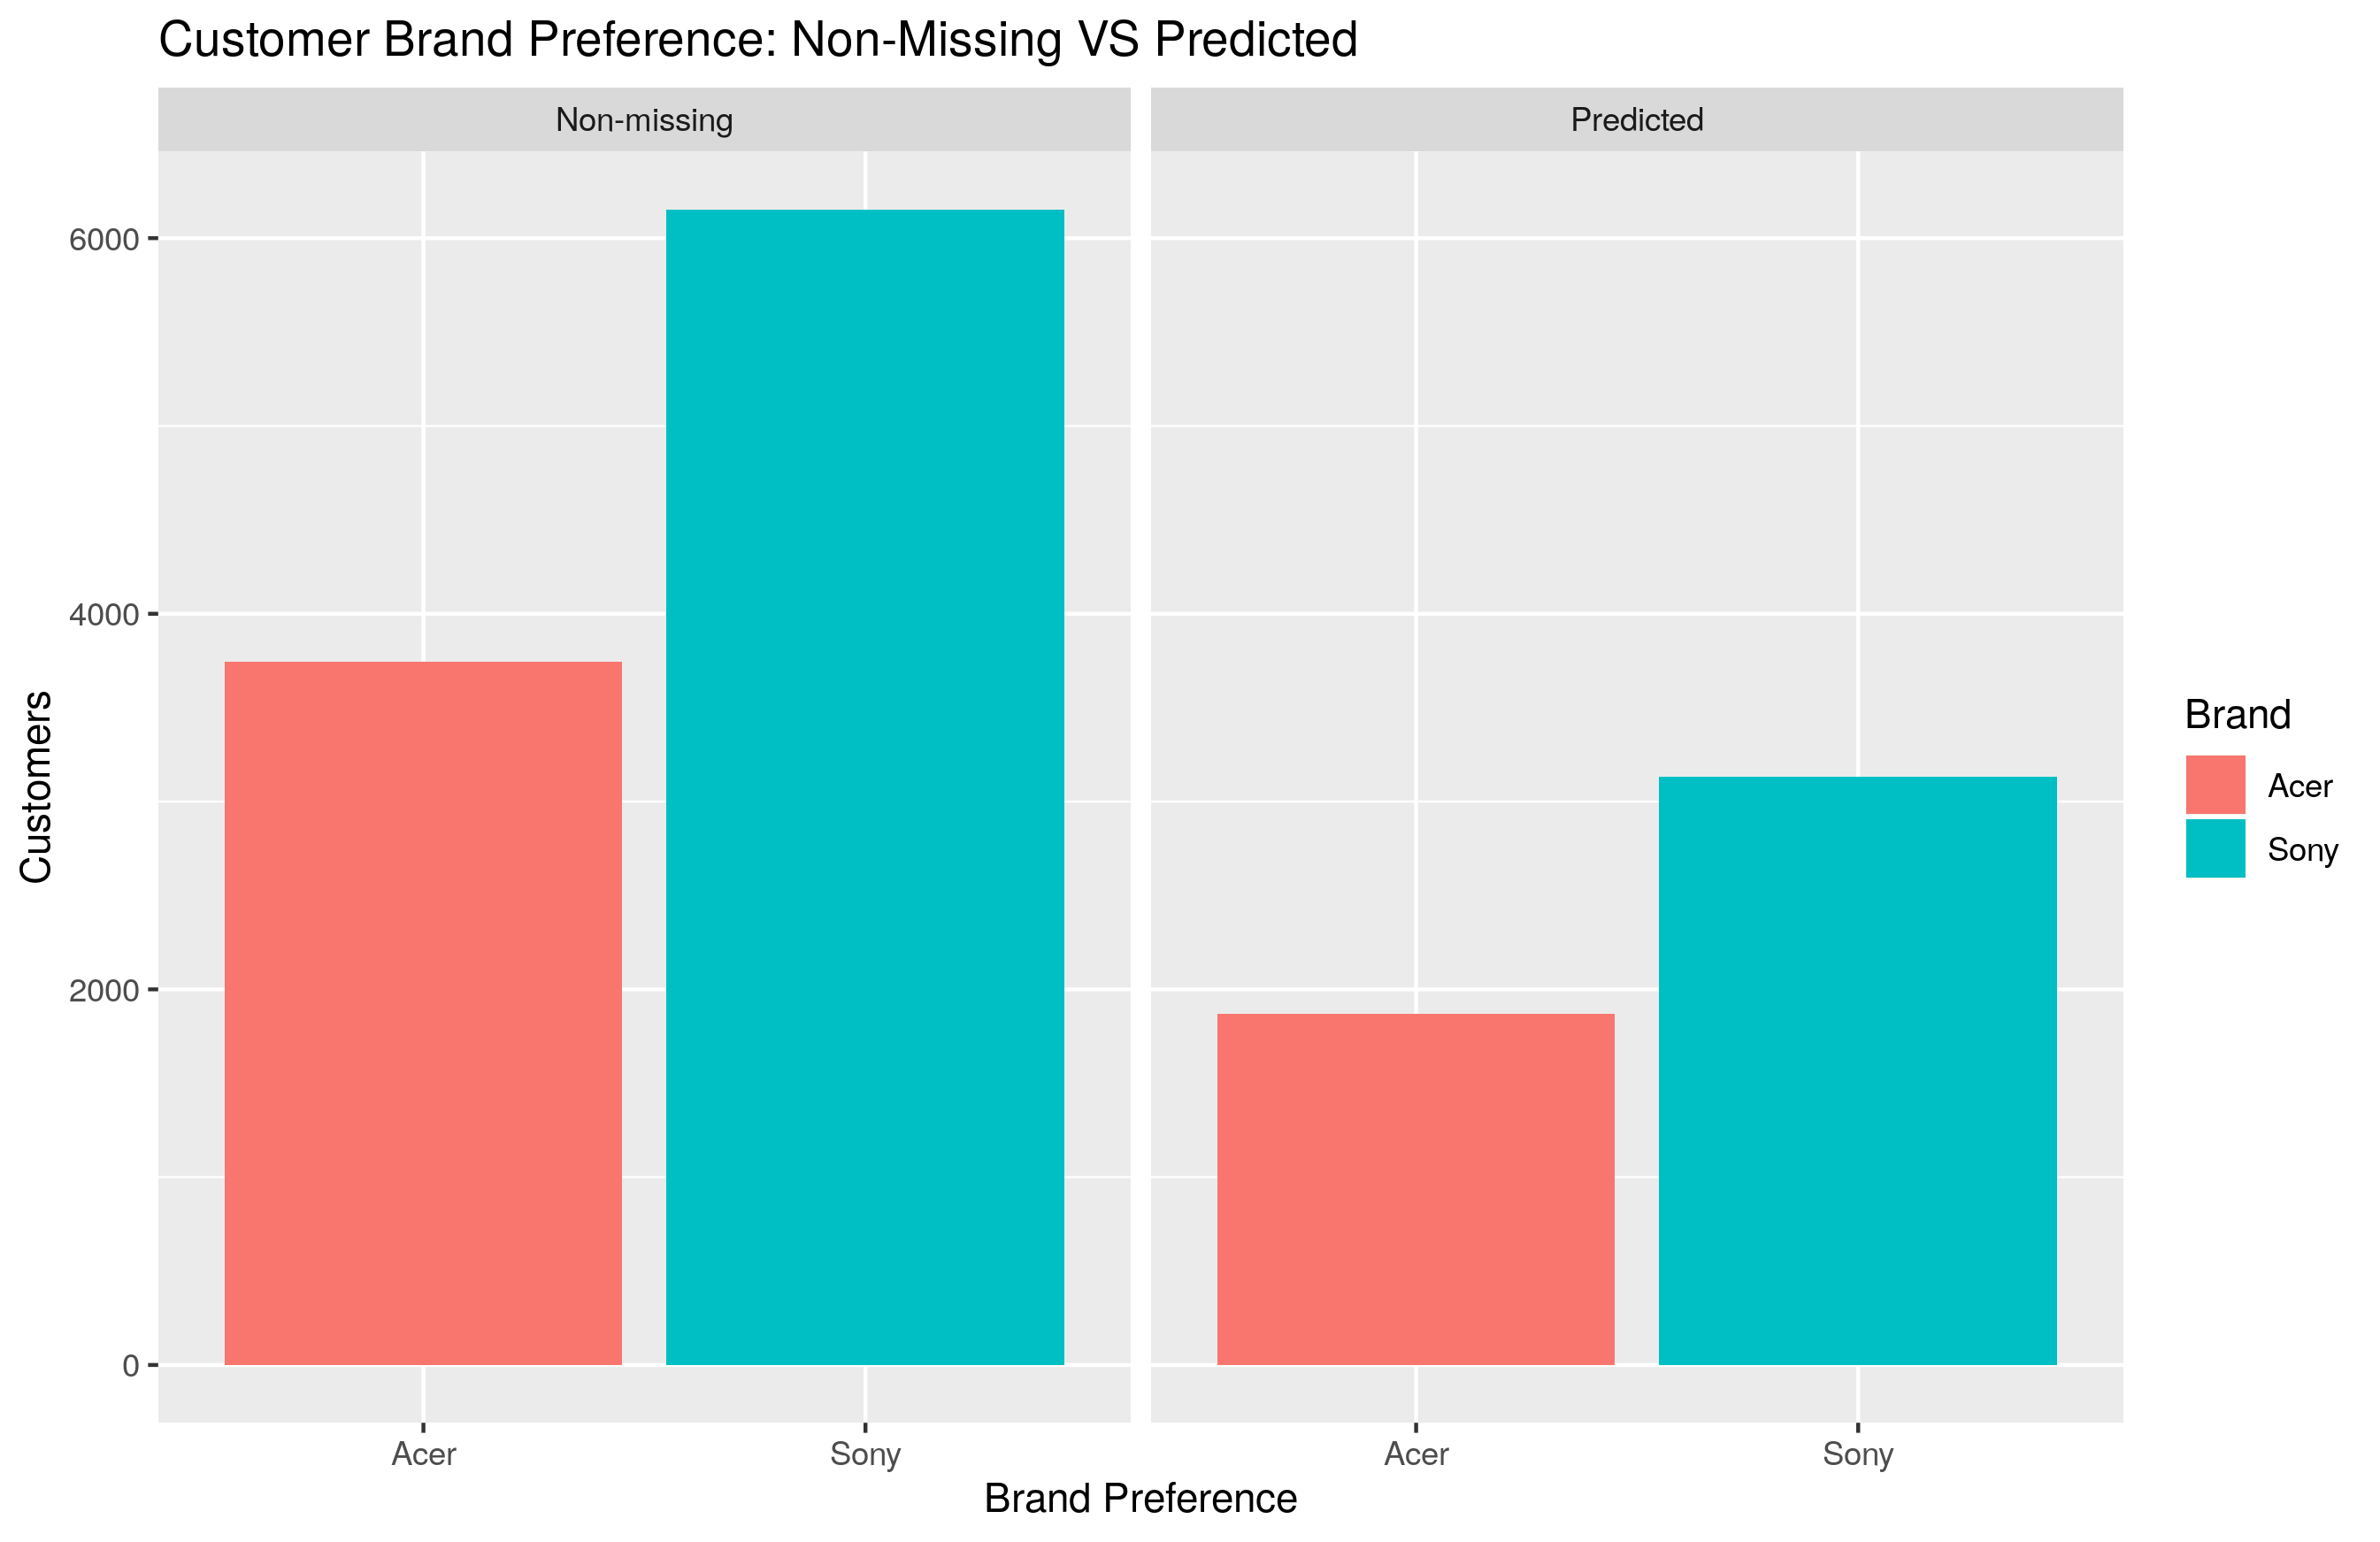
\includegraphics[width=\textwidth,height=\textheight,keepaspectratio]{brand_preference_marked.png}
    \par
}
\bigskip

We can see that the predicted values include a higher proportion of Acer preferences than there are in the data with values

\section{Chosen Model and Its' Performance}


\bigskip
{
    \centering
    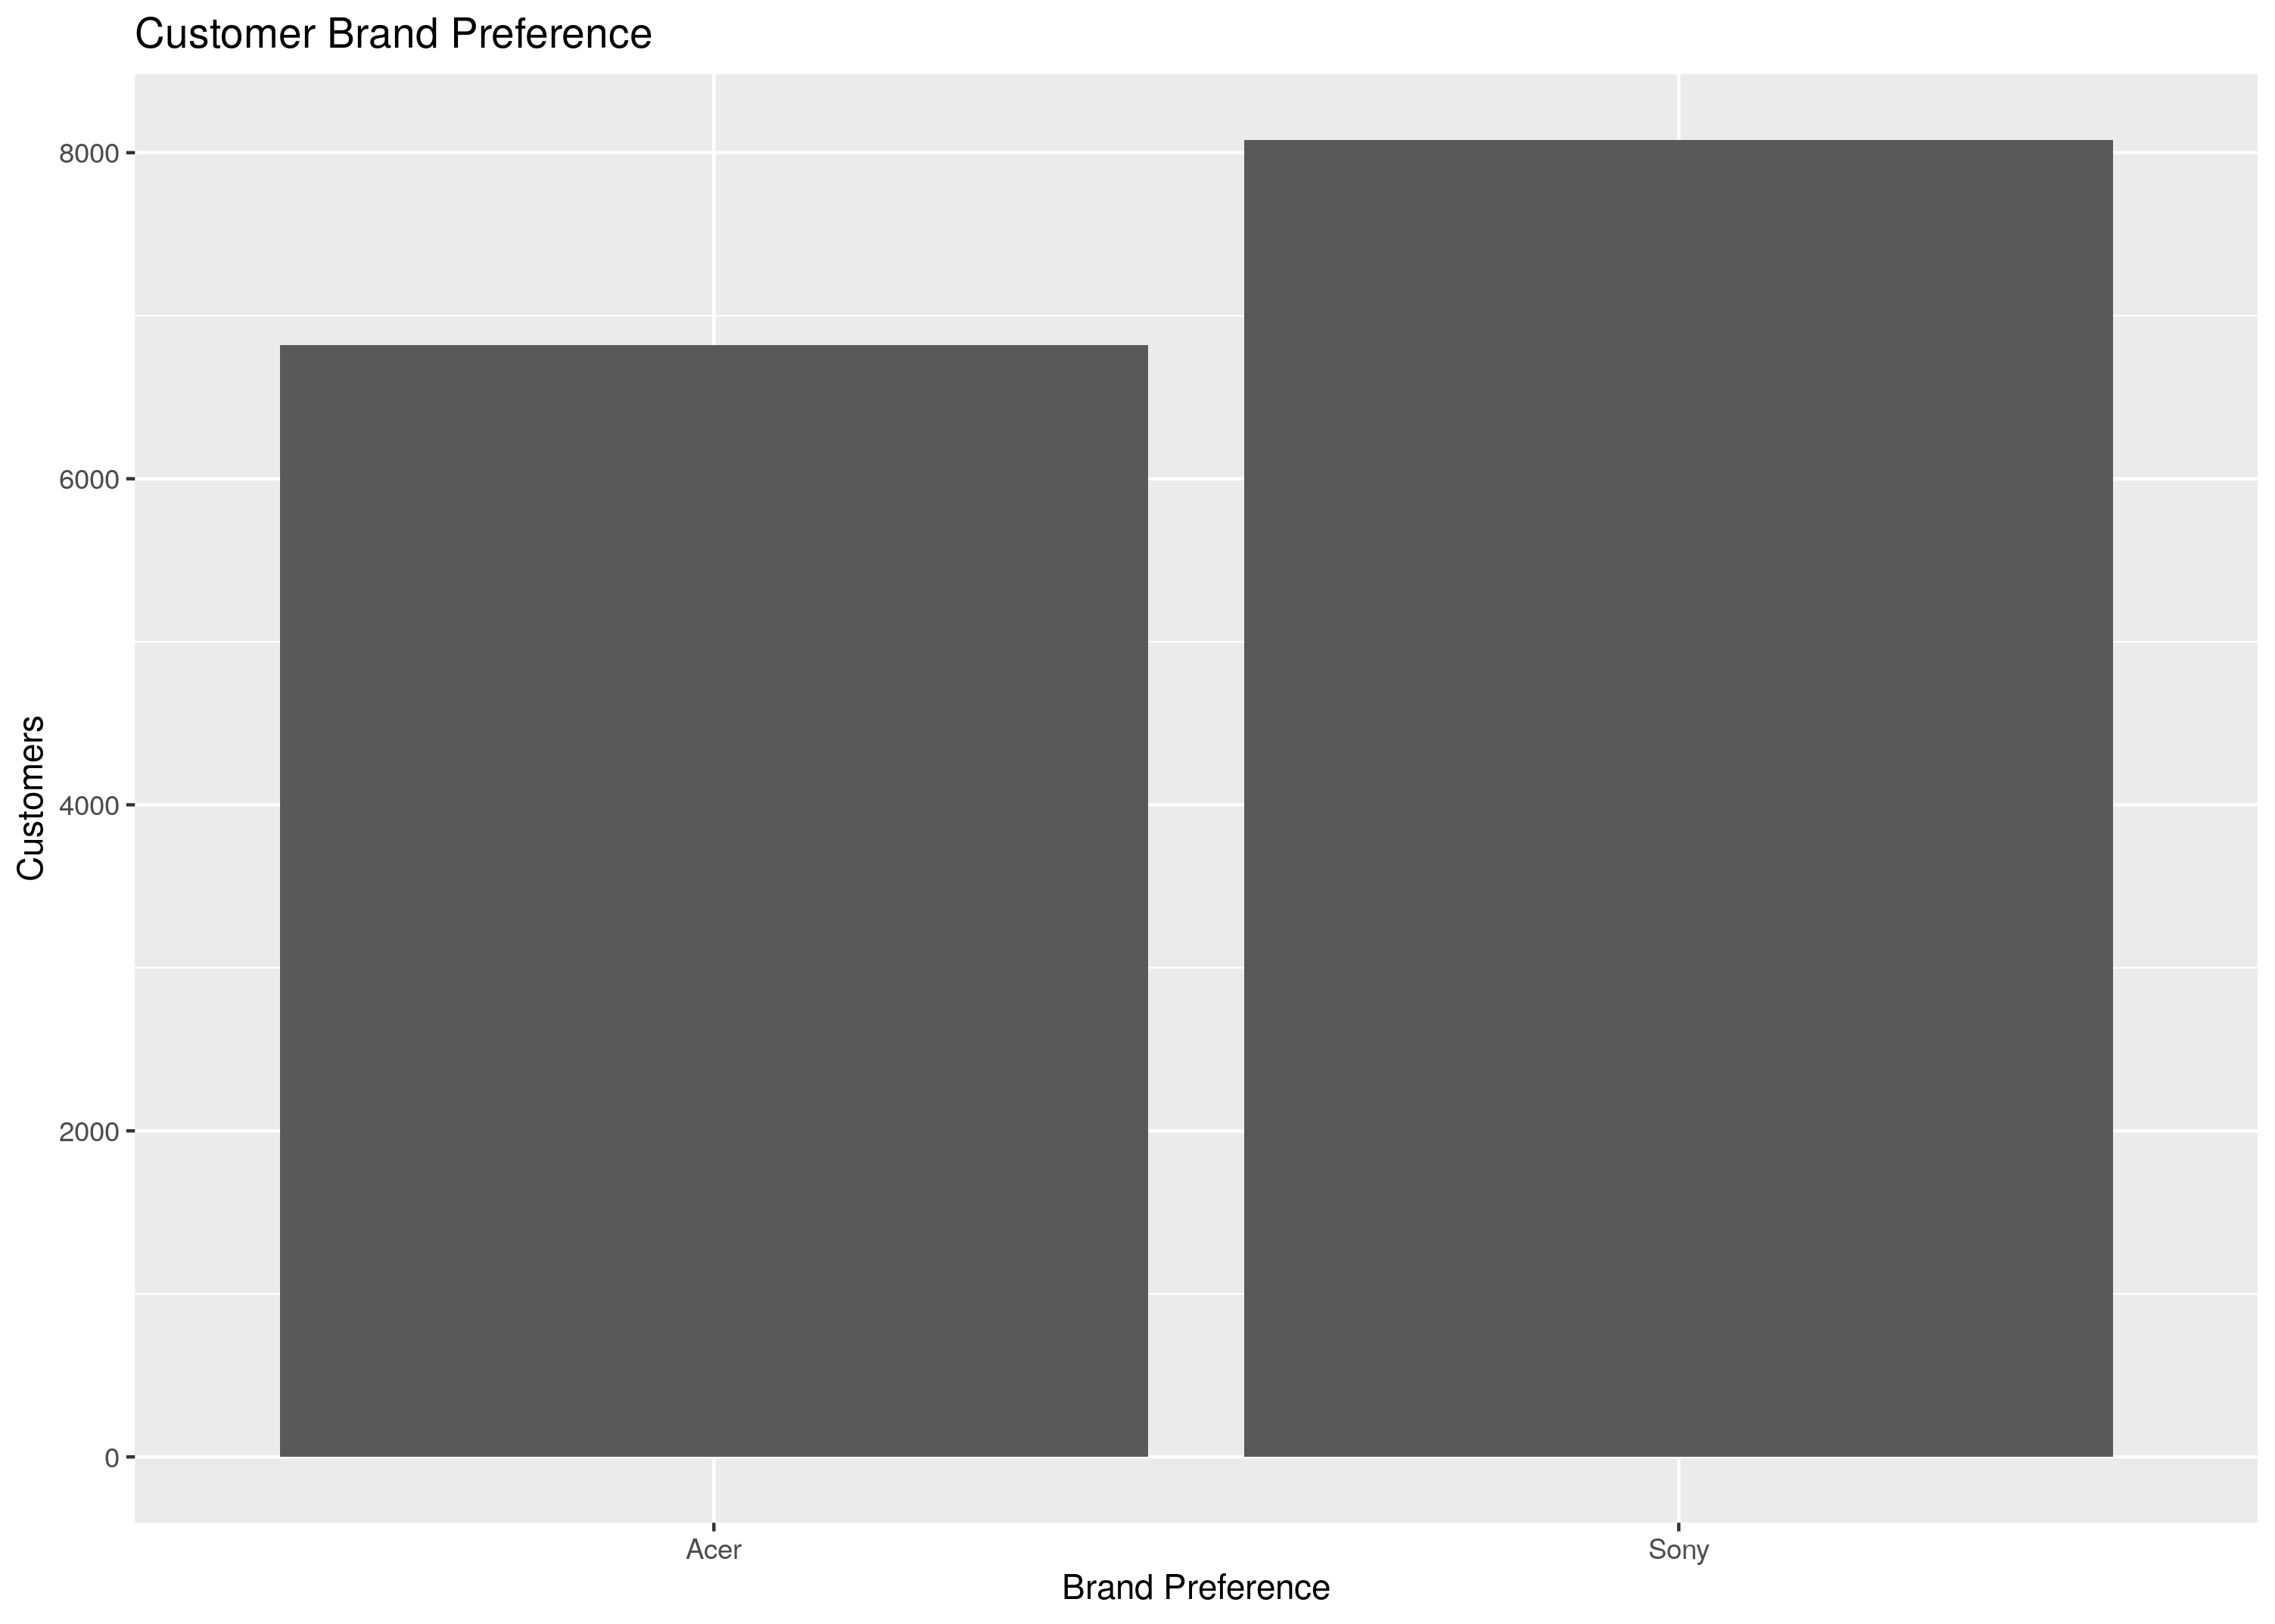
\includegraphics[width=\textwidth,height=\textheight,keepaspectratio]{brand_preference_plain.png}
    \par
}
\bigskip

Here we explain what is our model and how it performs


\section{Model Comparison and Performance}


\bigskip
{
    \centering
    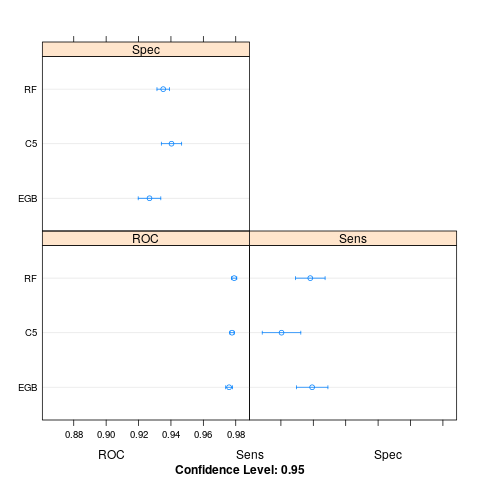
\includegraphics[width=\textwidth,height=\textheight,keepaspectratio]{dotplot_comparison.png}
    \par
}
\bigskip

\bigskip
{
    \centering
    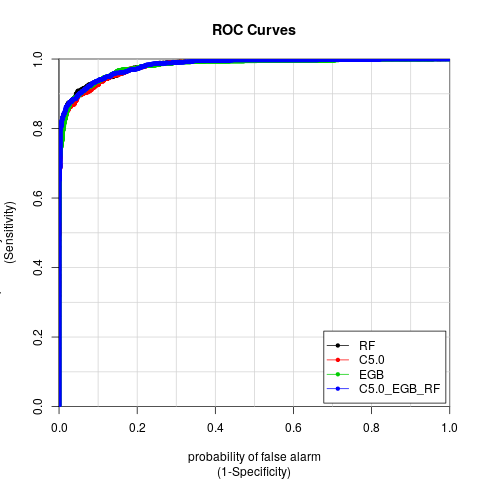
\includegraphics[width=\textwidth,height=\textheight,keepaspectratio]{AUC_comparison.png}
    \par
}
\bigskip

Differences between the models are very small

\bigskip
{
    \centering
    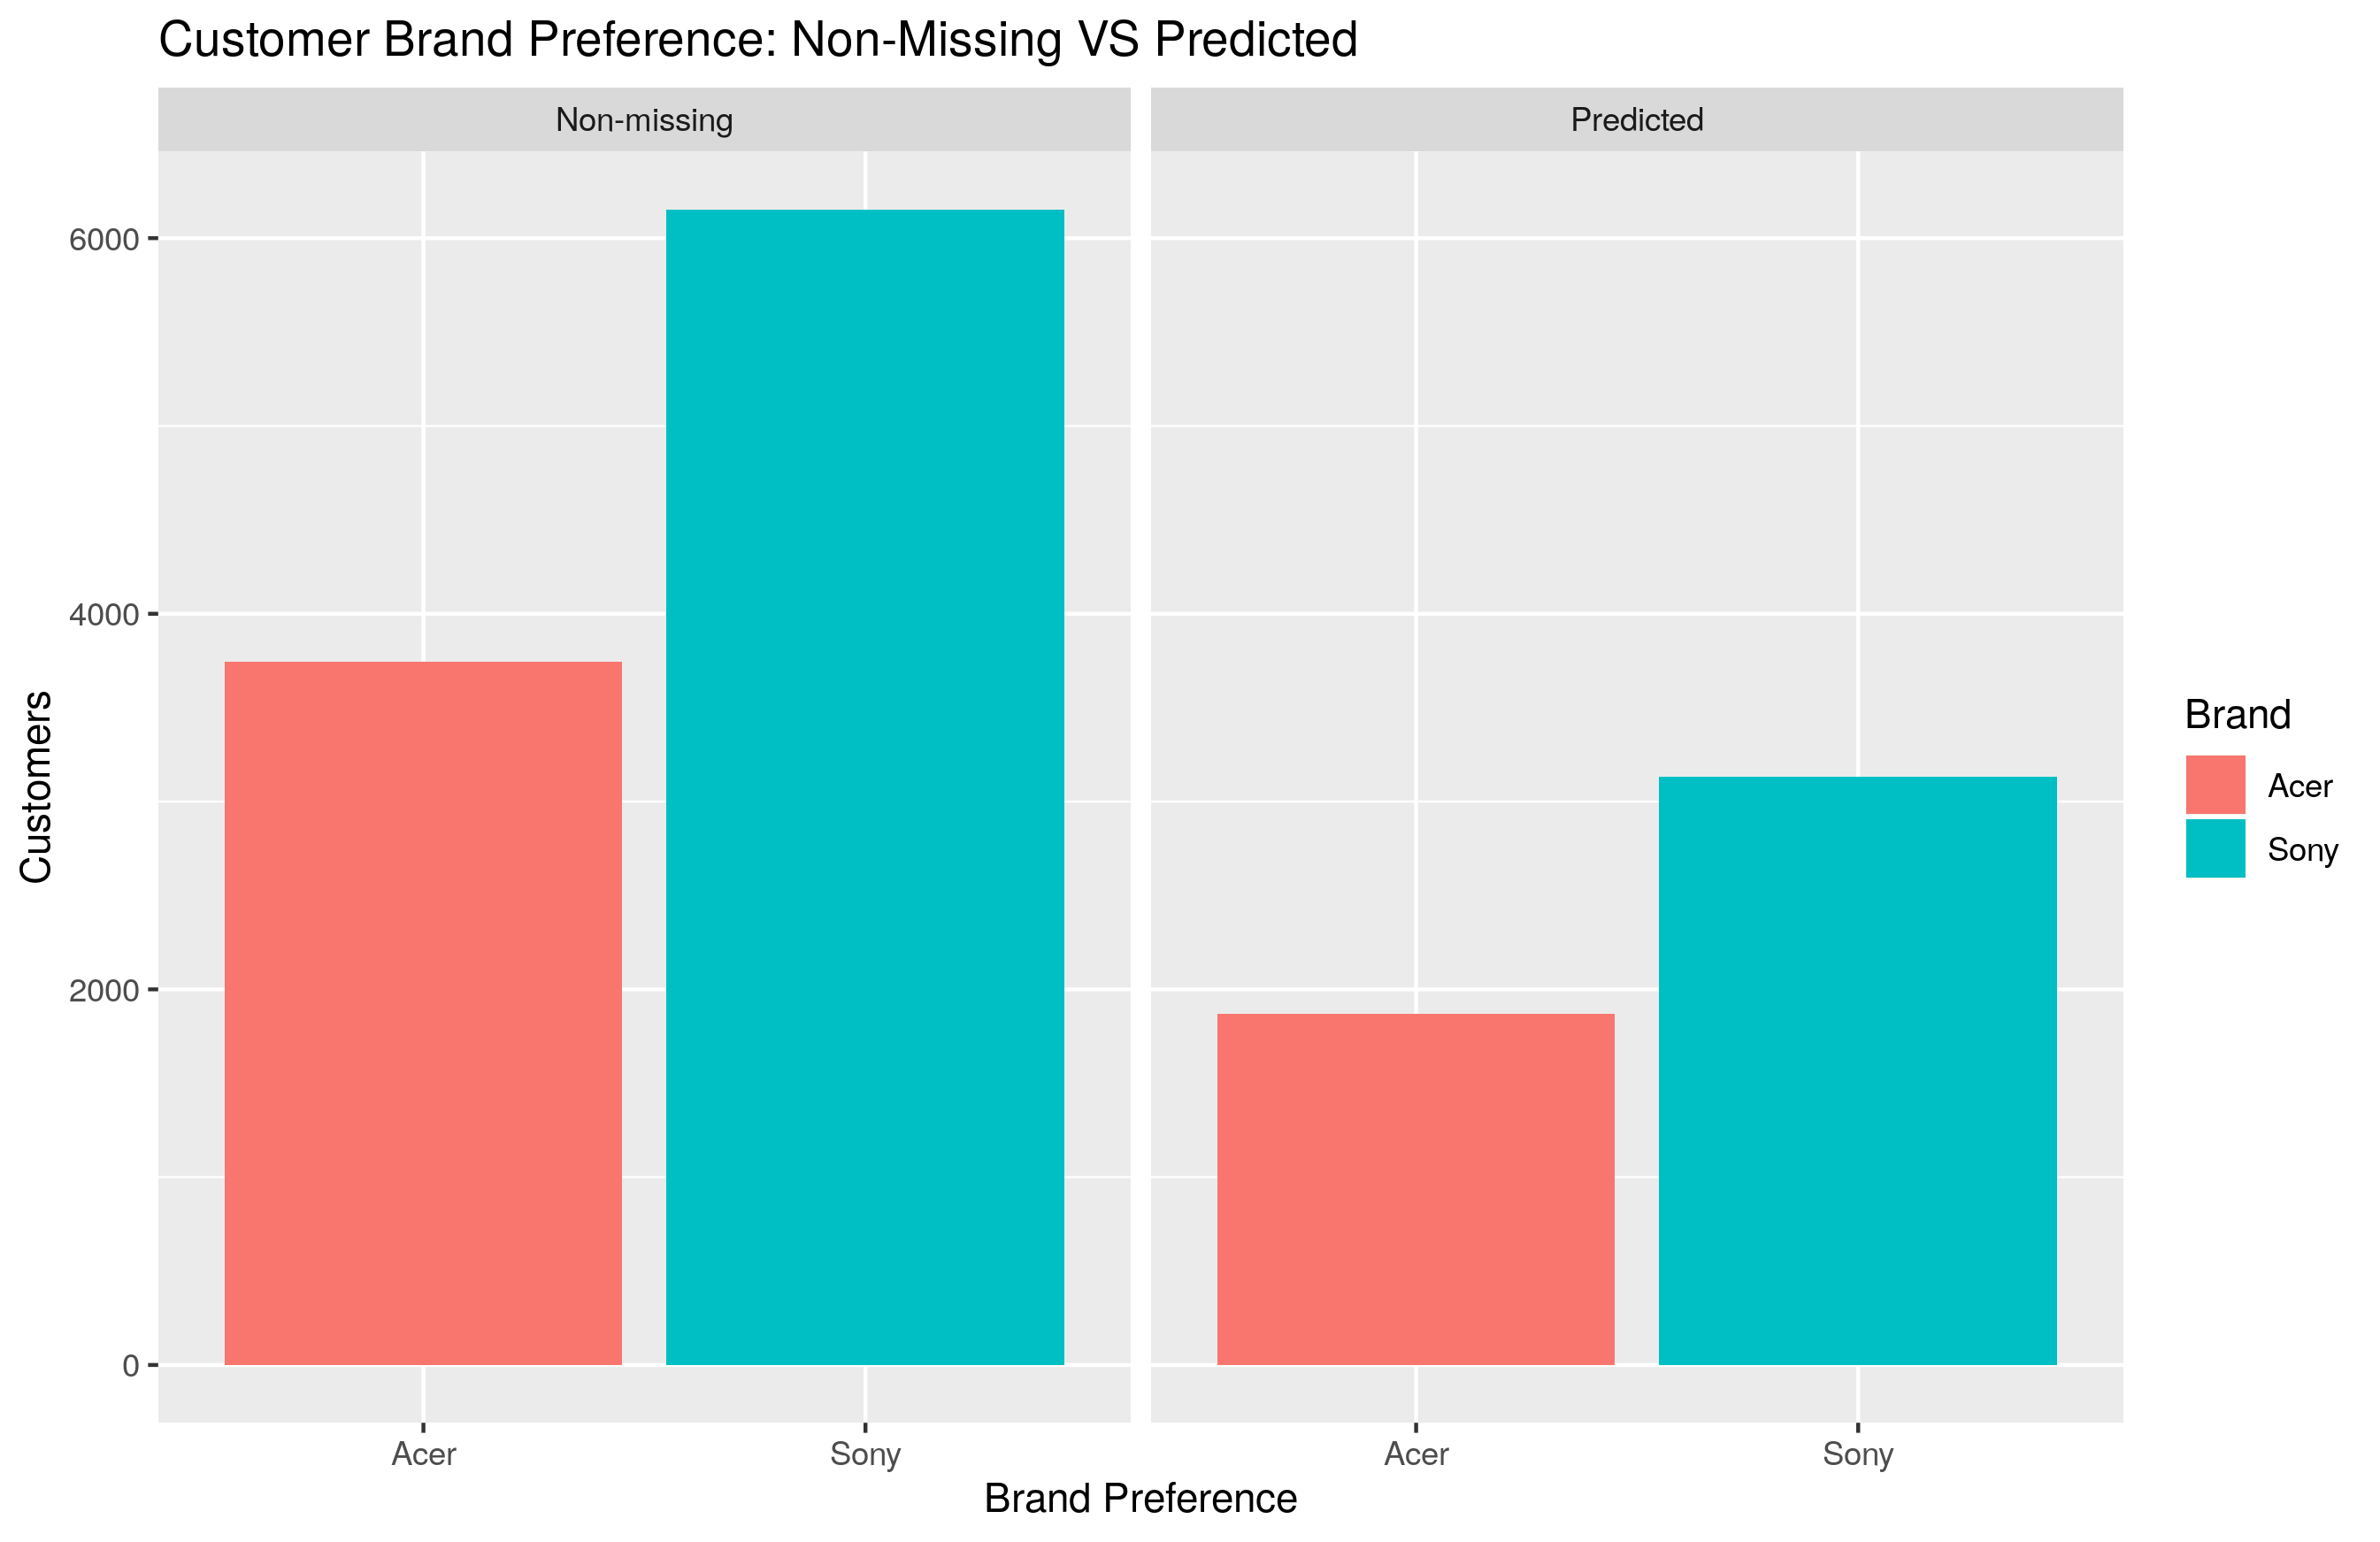
\includegraphics[width=\textwidth,height=\textheight,keepaspectratio]{model_prediction_correlations.png}
    \par
}
\bigskip


\lstinputlisting[float=h,frame=tb,caption=C5.0,label=zebra]{./figures/C5.0_output.txt}
\lstinputlisting[float=h,frame=tb,caption=Extreme Gradient Boosting,label=zebra]{./figures/EGB_output.txt}
\lstinputlisting[float=h,frame=tb,caption=Random Forest,label=zebra]{./figures/RF_output.txt}
\lstinputlisting[float=h,frame=tb,caption=GLM Ensemble (C5.0 + EGB + RF),label=zebra]{./figures/C5.0_EGB_RF_output.txt}

\end{document}
